\documentclass{beamer}
\usetheme{Madrid}
%\useoutertheme{miniframes} % Alternatively: miniframes, infolines, split
\useinnertheme{circles}

\definecolor{UBCblue}{rgb}{0.04706, 0.13725, 0.26667} % UBC Blue (primary)
\definecolor{UBCgrey}{rgb}{0.3686, 0.5255, 0.6235} % UBC Grey (secondary)

\setbeamercolor{palette primary}{bg=UBCblue,fg=white}
\setbeamercolor{palette secondary}{bg=UBCblue,fg=white}
\setbeamercolor{palette tertiary}{bg=UBCblue,fg=white}
\setbeamercolor{palette quaternary}{bg=UBCblue,fg=white}
\setbeamercolor{structure}{fg=UBCblue} % itemize, enumerate, etc
\setbeamercolor{section in toc}{fg=UBCblue} % TOC sections

% Override palette coloring with secondary
\setbeamercolor{subsection in head/foot}{bg=UBCgrey,fg=white}
\usepackage[T1]{fontenc}
\usepackage[polish]{babel}
\usepackage{xunicode}
\usepackage{xltxtra}
\usepackage{caption}
\usepackage{graphicx}
\usepackage{subcaption}
\usepackage{bookmark}



\title{AT5G45470 \& AT5G45480}
\subtitle{Czyli meandry niekodującego RNA}
\author{Konstancja Gałat}
\institute{BtMol II rok}
\date{\today}

\begin{document}

\begin{frame}
    \titlepage
\end{frame}

\begin{frame}
    \frametitle{Plan prezentacji}
    \tableofcontents
\end{frame}

\section{Wstęp}
\subsection{Genom \textit{Arabidopsis thaliana}}

\begin{frame}
    \frametitle{Genom Arabidopsis}
    \begin{figure}
        \centering
        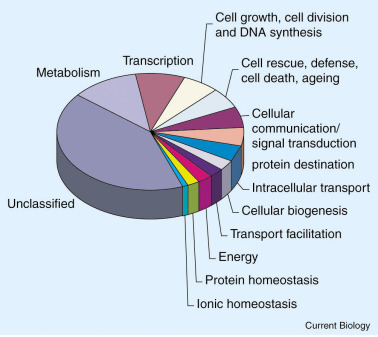
\includegraphics[scale=0.8]{functions.jpg}\\
        \scriptsize{10.1186/1741-7007-3-7}
    \end{figure}
\end{frame}

\subsection{\textit{Sporobolomyces ruberrimus}}
\begin{frame}
    \frametitle{\textit{Sporobolomyces ruberrimus}}
    \begin{figure}
        \centering
        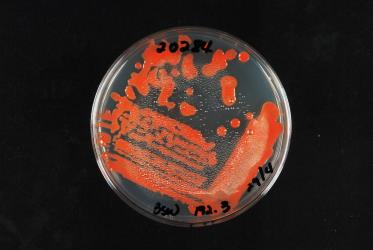
\includegraphics[scale=0.8]{sporobolo.jpg}\\
        \scriptsize{\textit{Sporobolomyces ruberrimus}\\
         Yamasaki $\&$ H. Fujii ex Fell, Pinel, Scorzetti, Statzell $\&$ Yarrow 2002}
    \end{figure}
\end{frame}

\begin{frame}
    \frametitle{\textit{Sporobolomyces ruberrimus}}
    \begin{figure}
    \begin{subfigure}{.5\textwidth}
    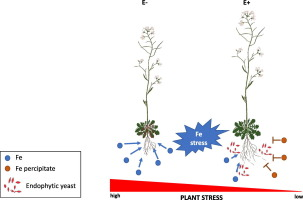
\includegraphics[scale=0.7]{romek.jpg}
    \end{subfigure}%
    \begin{subfigure}{.5\textwidth}
    \begin{flushleft}
    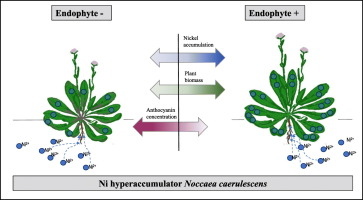
\includegraphics[scale = 0.7]{piotr.jpg}
    \end{flushleft}
    \end{subfigure}
\end{figure}

% \vspace*{\fill}
\vspace{1cm}
\scriptsize{10.1016/j.scitotenv.2023.161887\\
10.1016/j.scitotenv.2020.144666}
\end{frame}

\subsection{AT5G45472}
\begin{frame}
    \frametitle{AT5G45472}
    \begin{figure}
    \begin{subfigure}{.3\textwidth}
    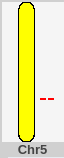
\includegraphics[width=.4\linewidth]{chromosom.png}
    \end{subfigure}%
    \begin{subfigure}{.7\textwidth}
    \begin{flushleft}
    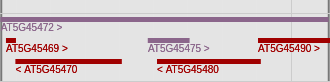
\includegraphics[scale = 0.7]{at5g45472.png}
    \end{flushleft}
    \end{subfigure}
\end{figure}

% \vspace*{\fill}
\vspace{1cm}
\scriptsize{https://rnacentral.org/rna/URS0000A77357/3702\\
https://gbrowse.arabidopsis.org/cgi-bin/gb2/gbrowse/arabidopsis/?name=AT5G45472.1}
\end{frame}

\subsection{AT5G45470 \& AT5G45480}
\begin{frame}
    \frametitle{AT5G45470 \& AT5G45480}
    \centering
    AT5G45470
    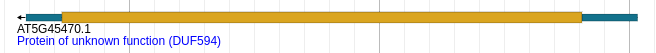
\includegraphics[scale = 0.5]{at5g45470.png}\\
    AT5G45480
    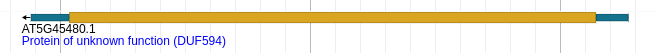
\includegraphics[scale = 0.5]{at5g45480.png}\\
    \hfill \break
    \scriptsize{https://jbrowse.arabidopsis.org/}
\end{frame}

\section{Białka}
\subsection{Proponowane struktury}
\begin{frame}
    \frametitle{Proponowane struktury}
    \begin{figure}
        \centering
    \begin{subfigure}{.5\textwidth}
        \centering
        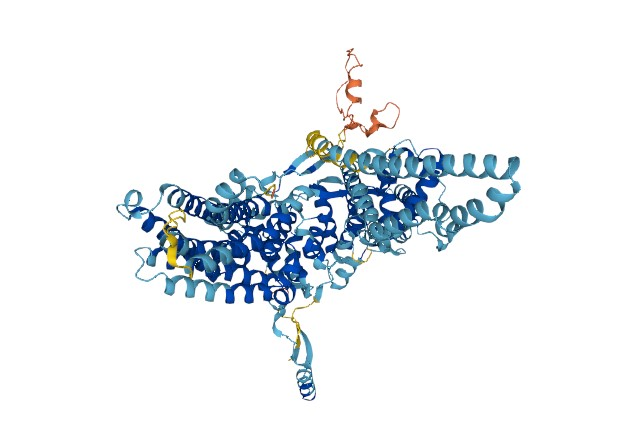
\includegraphics[scale = 0.5]{70img.jpg}
        \caption{Q9FHI9}
        \label{fig:70protein}
    \end{subfigure}%
    \begin{subfigure}{.5\textwidth}
        \centering
        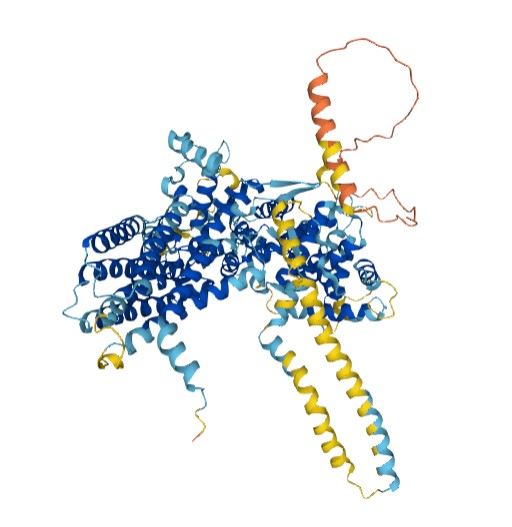
\includegraphics[scale = 0.5]{80img.jpg}
        \caption{Q9FHI8}
        \label{fig:80protein}
    \end{subfigure}
    \end{figure}
\end{frame}

\subsection{Porównanie struktur}
\begin{frame}
    \frametitle{Porównanie struktury białek}
    96.6\%!
    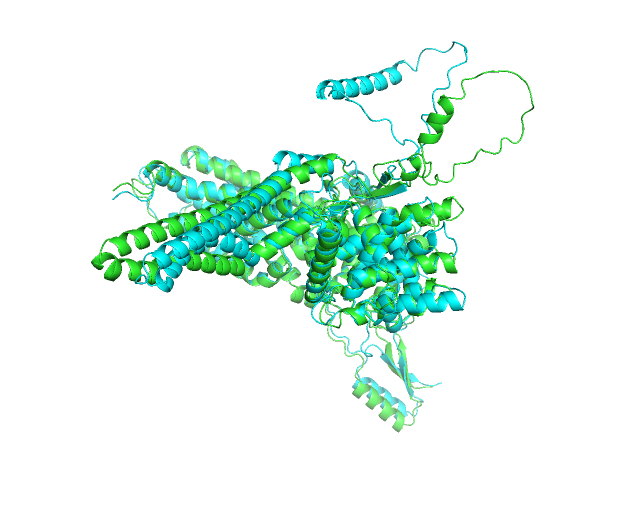
\includegraphics[scale=0.8]{nalozone.png}
\end{frame}

\begin{frame}
    \frametitle{DeepFRI}
    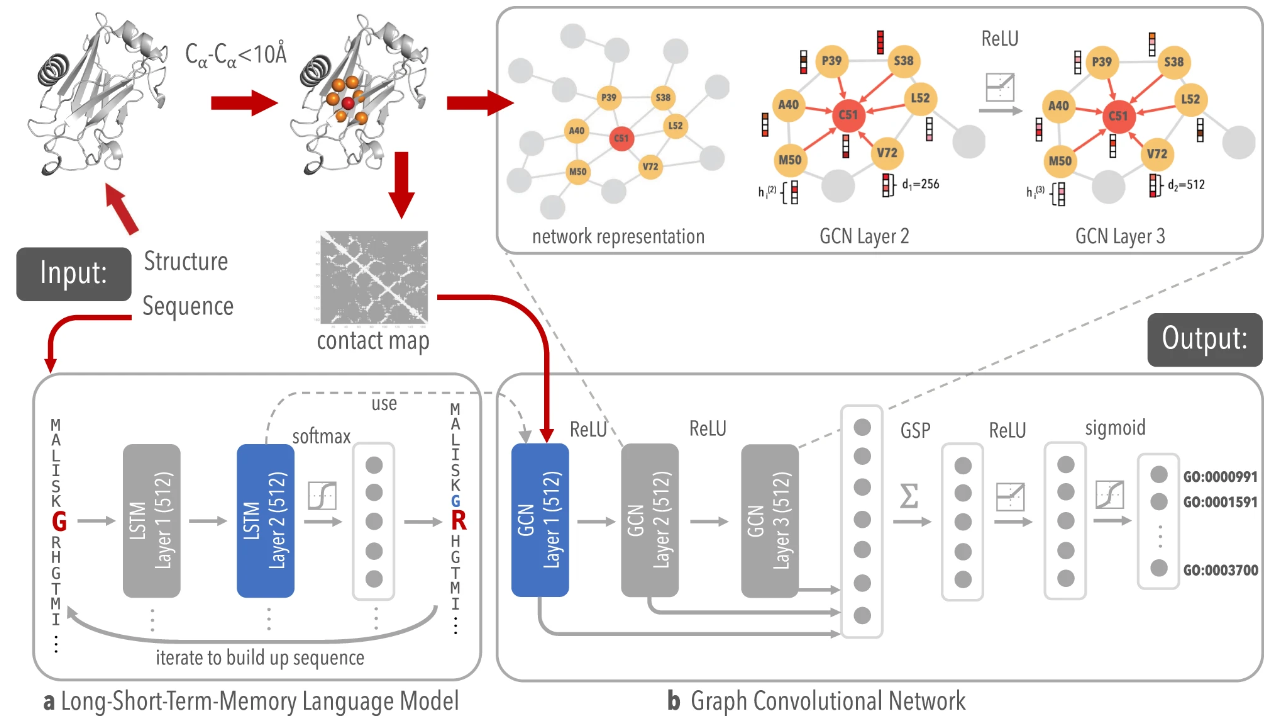
\includegraphics[scale=0.27]{deepfrischeme.png}
    \scriptsize{https://doi.org/10.5281/zenodo.4650027}
\end{frame}

\begin{frame}
    \frametitle{DeepFRI}
    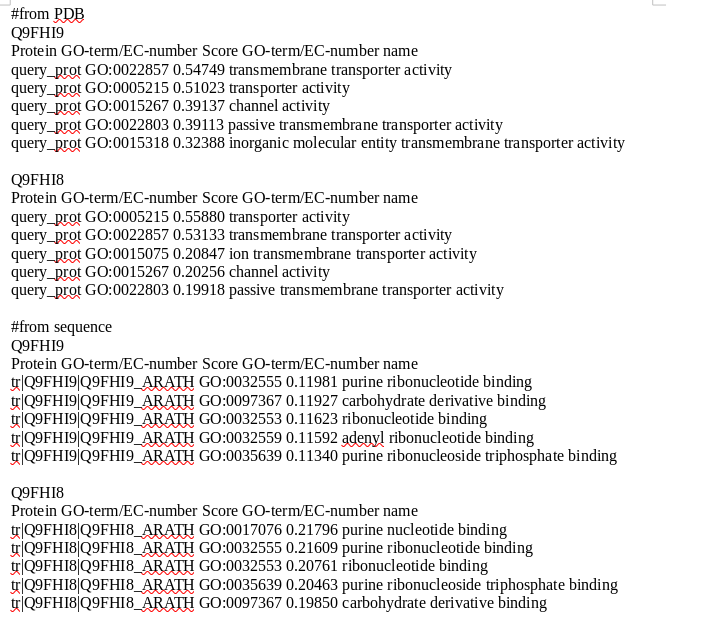
\includegraphics[scale=0.35]{deepfri.png}
\end{frame}

\section{Badania}

\subsection{Plan badań}
\begin{frame}
    \frametitle{Plan}
    \begin{enumerate}
        \item Transformacja \textit{A.thaliana}
        \item Analiza ekspresji AT5G45470 oraz AT5G45480
        \item Identyfikacja \textit{Sporobolomyces ruberrimus}
        \item Określenie lokalizacji komórkowej i tkankowej
        \item Analiza mutantów
    \end{enumerate}
\end{frame}

\subsection{Gateway}
\begin{frame}
    \frametitle{Wyniki}
    \begin{enumerate}
        \item Klonowanie metodą Gateway
        \item Hodowla \textit{A.thaliana} Col-0, w celu izolacji RNA (z oraz bez \textit{Sporobolomyces ruberrimus})
    \end{enumerate}
\end{frame}

\begin{frame}
    \frametitle{Gateway -- attb}
    \begin{figure}
        \centering
        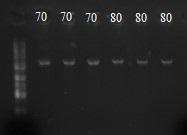
\includegraphics[scale=1.4]{zel1.jpg}\\
        \caption*\hfill{Produkty reakcji PCR ze starterami specyficznymi do sekwencji AT5G45470 oraz AT5G45480 -- powielone geny z dołączonymi sekwencjami attb}%
    \end{figure}
\end{frame}

\begin{frame}
    \frametitle{Gateway -- BP}
    \begin{figure}[!htb]
        \centering
        \subfloat[\centering]{{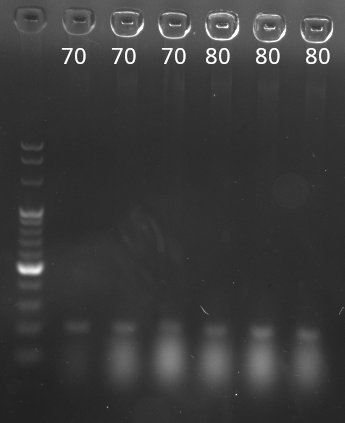
\includegraphics[scale = 1.2]{bp_gel_final.png} }}
        \qquad
        \subfloat[\centering]{{
\includegraphics[scale =0.2]{SadFaceEmoji.png} }}
        \caption*\hfill{\scriptsize a) Produkty kolonijnego PCR po reakcji BP b) PCR potwierdzający obecność wstawki w plazmidzie po reakcji BP}%
        \label{fig:zele2}
    \end{figure}
\end{frame}

\subsection{Identyfikacja grzyba}
\begin{frame}
    \frametitle{Identyfikacja grzyba}
    Analiza z wykorzystaniem BLAST wykazała, że sekwencją najbardziej komplementarną do
    sekwencjonowanej był fragment pochodzący z organizmu Sporobolomyces ruberrimus. Podobieństwo 
    to wynosiło 99.9\%, Spośród ok. 1300 nukleotydów tylko 1 został nierozpoznany. To
    pozwala sądzić, że rośliny inokulowano grzybem Sporobolomyces ruberrimus.
\end{frame}

\subsection{qPCR}
\begin{frame}
    \frametitle{qPCR}
    \begin{figure}
        \centering
        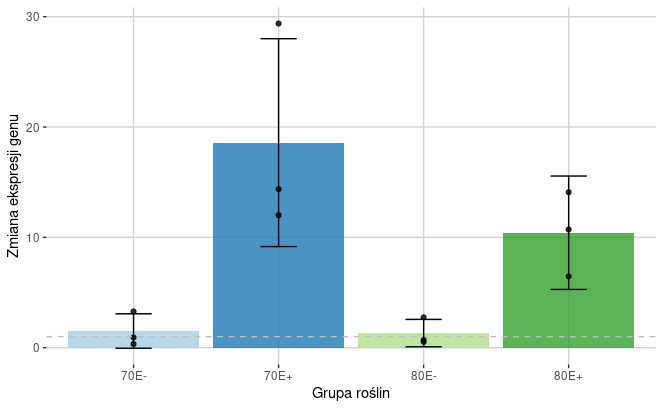
\includegraphics[scale=0.4]{qpcr.png}\\
        \caption*\hfill{\scriptsize Kiełkowanie roślin w czasie}%
    \end{figure}
    \small Wykazano różnice istotnie statystyczne dla obydwu genów.
\end{frame}

\subsection{Hodowla wazonowa}
\begin{frame}
    \frametitle{Hodowla wazonowa -- AT5G45470}
    \begin{figure}
        \centering
        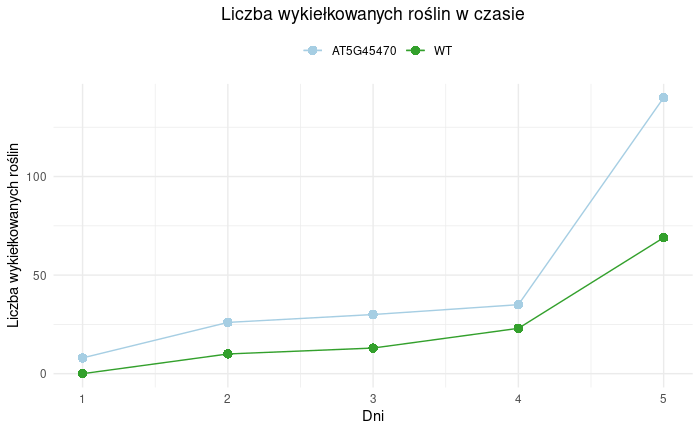
\includegraphics[scale=0.4]{kielkowanie1.png}\\
        \caption*\hfill{\scriptsize Kiełkowanie roślin w czasie}%
    \end{figure}
    \small Wykazano brak różnic istotnych statystycznie, ale eksperyment zostanie powtórzony.
\end{frame}

\begin{frame}
    \frametitle{Hodowla wazonowa -- AT5G45470}
    \begin{figure}
        \centering
        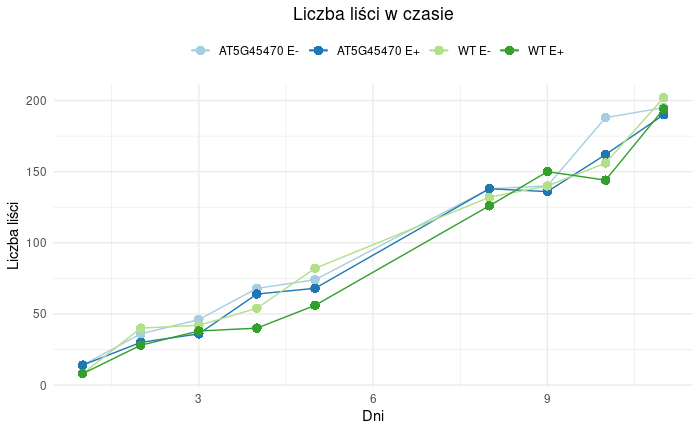
\includegraphics[scale=0.5]{liscie1.png}\\
        \caption*\hfill{\scriptsize Ilość liści roślin w czasie}%
    \end{figure}
    \small Wykazano brak różnic istotnych statystycznie (ANOVA).
\end{frame}

\begin{frame}
    \frametitle{Hodowla wazonowa -- AT5G45470}
    \begin{figure}
        \centering
        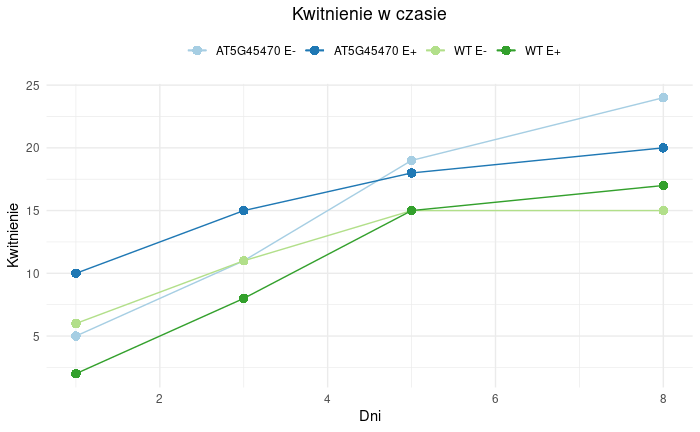
\includegraphics[scale=0.5]{kwit1.png}\\
        \caption*\hfill{\scriptsize Kwitnienie roślin w czasie}%
    \end{figure}
    \small Wykazano różnicę istotną statystycznie między WT E+ i AT5G45470 E+ (ANOVA).
\end{frame}

\begin{frame}

    Dziękuję za uwagę!

\end{frame}
\end{document}

